%%%%%%%%%%%%%%%%%%%%%%%%%%%%%%%%%%%%%%%%%
% Journal Article
% LaTeX Template
% Version 1.4 (15/5/16)
%
% This template has been downloaded from:
% http://www.LaTeXTemplates.com
%
% Original author:
% Frits Wenneker (http://www.howtotex.com) with extensive modifications by
% Vel (vel@LaTeXTemplates.com)
%
% License:
% CC BY-NC-SA 3.0 (http://creativecommons.org/licenses/by-nc-sa/3.0/)
%
%%%%%%%%%%%%%%%%%%%%%%%%%%%%%%%%%%%%%%%%%

%----------------------------------------------------------------------------------------
%	PACKAGES AND OTHER DOCUMENT CONFIGURATIONS
%----------------------------------------------------------------------------------------

\documentclass[twoside,twocolumn]{article}

\usepackage[sc]{mathpazo} % Use the Palatino font
\usepackage[T1]{fontenc} % Use 8-bit encoding that has 256 glyphs
\linespread{1.05} % Line spacing - Palatino needs more space between lines
\usepackage{microtype} % Slightly tweak font spacing for aesthetics

\usepackage[english]{babel} % Language hyphenation and typographical rules

\usepackage[hmarginratio=1:1,top=32mm,columnsep=20pt]{geometry} % Document margins
\usepackage[hang, small,labelfont=bf,up,textfont=it,up]{caption} % Custom captions under/above floats in tables or figures
\usepackage{booktabs} % Horizontal rules in tables

\usepackage{lettrine} % The lettrine is the first enlarged letter at the beginning of the text

\usepackage{enumitem} % Customized lists
\setlist[itemize]{noitemsep} % Make itemize lists more compact

\usepackage{abstract} % Allows abstract customization
\renewcommand{\abstractnamefont}{\normalfont\bfseries} % Set the "Abstract" text to bold
\renewcommand{\abstracttextfont}{\normalfont\small\itshape} % Set the abstract itself to small italic text

\usepackage{titlesec} % Allows customization of titles
\renewcommand\thesection{\Roman{section}} % Roman numerals for the sections
\renewcommand\thesubsection{\roman{subsection}} % roman numerals for subsections
\titleformat{\section}[block]{\large\scshape\centering}{\thesection.}{1em}{} % Change the look of the section titles
\titleformat{\subsection}[block]{\large}{\thesubsection.}{1em}{} % Change the look of the section titles

\usepackage{fancyhdr} % Headers and footers
\pagestyle{fancy} % All pages have headers and footers
\fancyhead{} % Blank out the default header
\fancyfoot{} % Blank out the default footer
\fancyhead[C]{} % Custom header text
\fancyfoot[RO,LE]{\thepage} % Custom footer text

\usepackage{titling} % Customizing the title section

\usepackage{hyperref} % For hyperlinks in the PDF
\usepackage{amsmath}
\usepackage[rightcaption]{sidecap}
 \usepackage{gensymb}
\usepackage{graphicx} %package to manage images
\graphicspath{{images/} }
%----------------------------------------------------------------------------------------
%	TITLE SECTION
%----------------------------------------------------------------------------------------

\setlength{\droptitle}{-4\baselineskip} % Move the title up

\pretitle{\begin{center}\Huge\bfseries} % Article title formatting
\posttitle{\end{center}} % Article title closing formatting
\title{Array lineare di antenna a microstriscia per applicazioni IEEE 802.11} % Article title
\author{%
\textsc{Francesco Morgillo}\\[1ex] % Your name
\normalsize Università degli studi di Genova \\ % Your institution
\normalsize \href{mailto:francesco.morgillo@hotmail.com}{francesco.morgillo@hotmail.com} % Your email address
%\and % Uncomment if 2 authors are required, duplicate these 4 lines if more
%\textsc{Jane Smith}\thanks{Corresponding author} \\[1ex] % Second author's name
%\normalsize University of Utah \\ % Second author's institution
%\normalsize \href{mailto:jane@smith.com}{jane@smith.com} % Second author's email address
}
\date{\today} % Leave empty to omit a date
\renewcommand{\maketitlehookd}{%

\begin{abstract}
\noindent Design of a patch antenna linear array for IEEE 802.11 wireless based application. % Dummy abstract text - replace \blindtext with your abstract text
\end{abstract}
}
%----------------------------------------------------------------------------------------

\begin{document}

\renewcommand{\refname}{Bibliografia}
% Print the title
\maketitle

%----------------------------------------------------------------------------------------
%	ARTICLE CONTENTS
%----------------------------------------------------------------------------------------

\section{Introduzione}


Si vuole progettare un array lineare Broadside di 4 antenne a micro-striscia (patch), destinata ad applicazioni Wireless IEEE 802.11.
L'antenna dovrà operare nella banda 2400 – 2500 MHz utilizzata nelle applicazioni Wi-Fi.
Dai requisiti appena riportati, ricaviamo le seguenti specifiche per l'antenna

\begin{enumerate}[noitemsep] % [noitemsep] removes whitespace between the items for a compact look
\item Frequenza centrale: 2.45 GHz
\item Banda: 100 MHz
\item Guadagno:  
\end{enumerate}
 e per l'array
 \begin{enumerate}[noitemsep] % [noitemsep] removes whitespace between the items for a compact look
\item Numero di elementi:4 
\item Tipo schiera: Lineare, Broadside
\end{enumerate}

%------------------------------------------------


\section{Singolo elemento}
Il singolo elemento dell'array è costituito da un'antenna a micro-striscia rettangolare.
Viene realizzata su di un substrato di materiale dielettrico, su cui viene fotoinciso uno strato conduttivo di lunghezza L e larghezza W. Sulla faccia opposta del substrato viene posto un piano di massa. L'elemento radiante può essere alimentato in diversi modi: per esempio tramite una linea realizzata in micro-striscia che raggiunge il bordo della patch, oppure con una sonda coassiale che attraversa il substrato.
\subsection*{Geometria}
Il dimensionamento della patch richiede l'impiego di equazioni ricavate con metodi numerici o empirici che tengono conto di effetti fisici dovuti alla complessità e non idealità dell'antenna.
Innanzitutto è necessario tenere presente che per via degli effetti ai bordi, le linee di campo della micro-striscia attraversano due dielettrici differenti, l'aria e il substrato.E' necessario quindi considerare una costante di conducibilità elettrica effettiva $\epsilon_{{reff}}$ che otteniamo è data da 
\begin{equation}
\label{eq:emc}
\epsilon_{reff}= \frac{\epsilon_{r}+1}{2}+\frac{\epsilon_{r}-1}{2}\Big[1+12\frac{h}{W}\Big]^{-\frac{1}{2}}
\end{equation}

Questa quantità corrisponde alla conducibilità elettrica di un materiale dielettrico omogeneo in cui si assume di immergere il modello della microstriscia.

\begin{figure}
  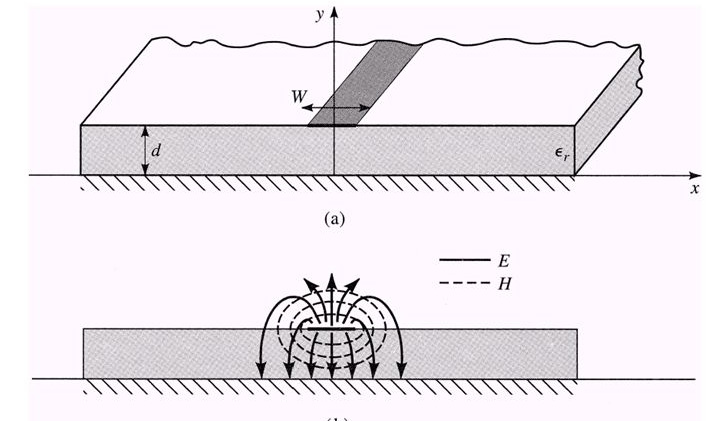
\includegraphics[width=\linewidth]{MICROSTRIPlinefield.jpg}
  \caption{Linee di campo E ed H di una microstriscia.}
  \label{fig:linefield}
\end{figure}
L'effetto ai bordi è poco influente dato che in linea generale \(L/h\gg 1\), ma non può essere ignorato dato che influisce sulla frequenza risonante dell'antenna.


Sempre a causa dell'effetto ai bordi, la lunghezza dell'antenna risulta elettricamente maggiore rispetto alla dimensione reale.
Il campo elettrico che curva attorno le aperture allunga elettricamente ogni lato di una quantità $\Delta L$ .
Un'approssimazione di questa quantità è data da

\begin{equation}
\frac{\Delta L}{h}= 0.412\frac{(\epsilon_{reff}+0.3)\Big(\frac{W}{h}+0.264\Big)}{(\epsilon_{reff}-0.258)\Big(\frac{W}{h}+0.8\Big)}
\end{equation}

Si ha quindi che

\begin{equation}\label{eq:L}
L_{eff}=L+2\Delta L
\end{equation}
dove $L=\lambda/2$ per il modo dominante $TM_{010}$ senza effetto ai bordi.
La frequenza di risonanza è funzione della lunghezza dell'antenna e considerando l'effetto ai bordi è 
\begin{equation} \label{eq:freq}
f_{r(010)}=\frac{1}{2L_{eff}\sqrt{\epsilon_{reff}}\sqrt{\mu_{0}\epsilon_{0}}}
\end{equation}

La larghezza W dell'antenna patch è data da 
\begin{equation}
W=\frac{1}{2f_{r}\sqrt{\mu_{0}\epsilon_{0}}}\sqrt{\frac{2}{\epsilon_{r}+1}}
\end{equation}
mentre combinando la \eqref{eq:freq} e la \eqref{eq:L} si può ricavare la lunghezza L della patch

\begin{equation}
L=\frac{1}{2f_{r}\sqrt{\mu_{0}\epsilon_{0}}\sqrt{\epsilon_{reff}}}-2\Delta L
\end{equation}

Note la frequenza centrale $f_{r}= 2.45GHz$, e considerato il  
substrato di spessore h di 1.6 mm ed $\epsilon_{r}=4.4$,
si ricavano i valori

\begin{center}
\begin{tabular}{ |c|c| } 
 \hline
 W & 37.3 mm \\ 
 L & 27.8 mm \\ 
 $\epsilon_{reff}$ & 4.01 \\
 \hline
\end{tabular}
\end{center}

\subsection*{Adattamento di impedenza}
Il metodo più semplice per studiare l'impedenza dell'antenna a micro-striscia è quello di analizzare il suo modello come linea di trasmissione.
L'antenna viene vista quindi come una linea di trasmissione i cui estremi (che corrispondono agli "slot" radianti ai bordi della patch) sono modellati come  due paralleli RC.
I due slot sono identici con ammettenza $Y_{1}=G_{1}+jB_{1}$. Inoltre l'ammettenza totale è puramente reale, data dal parallelo delle due conduttanze  $Y_{in}=Y_{1}+Y_{2}=2G_{1}$ (per via di una "trasformazione di ammettenza"vedi balanis).
Per ricavare il valore di $G_{1}$ si fa riferimento all'equazione 
\begin{equation}
G_{1}= \frac{I_{1}}{120\pi}
\end{equation}
dove 
\begin{align*}
I_{1}= \int_0^\pi \Big[\dfrac{sin (\big( \frac{k_{0}W}{2} cos\theta\big)}{cos\theta}\Big]^2 sin^3\theta d\theta = \\
=-2+cos(X)+XS_{i}(X)+\frac{sinX}{X}
\end{align*}
con 
\begin{equation}
X=k_{0}W
\end{equation}

Nota $G_{1}$ si può dedurre la resistenza in ingresso $R_{in}$ della patch dato che 
\begin{equation}
R_{in}=Z_{in}= \frac{1}{Y_{in}}=\frac{1}{2G_{1}}
\end{equation}

Si modifica questa espressione in modo tale da considerare gli effetti di accoppiamento fra i due slot.

\begin{equation}
R_{in}=Z_{in}= \frac{1}{Y_{in}}=\frac{1}{2G_{1}+2G_{12}}
\end{equation}
Il valore di conduttanza mutua si approssima con 
\begin{equation}
G_{12}= \frac{1}{120\pi^2}\int_0^\pi \Big[\dfrac{sin (\big( \frac{k_{0}W}{2} cos\theta\big)}{cos\theta}\Big]^2 J_{0}(k_{0}Lsin\theta)sin^3\theta d\theta
\end{equation}

Si ottiene quindi l'impedenza in ingresso $R_{in}= 321.42$ per via numerica.
Scegliendo di alimentare la patch sul bordo (edge feed), con una linea a microstriscia, sarà necessario raggiungere il punto di alimentazione con una linea adattata a $R_{in}$.
Si può altrimenti scegliere di cambiare il punto di alimentazione spostandosi verso il centro della patch (inset feed), cercando il valore di impedenza più adatto.
Si è scelto come primo tentativo per alimentare l'elemento singolo di realizzare un inset feed, calcolando numericamente il valore $y_{0}$ in cui l'impedenza $R_{in}(y=y_{0})= 50 \; \Omega$, ovvero un carico adattato alla linea di alimentazione.
Sapendo che 

\begin{align} \label{eq:Rin}
\begin{split}
R_{in}(y=y_{0})=\frac{1}{2(G_{1}+G_{12})}cos^2\Big( \frac{\pi}{L}y_{0}\Big)=\\
=R_{in}(y=0)cos^2\Big(\frac{\pi}{L}y_{0}\Big)
\end{split}
\end{align}

Risolvendo per $y_{0}$ e imponendo \newline$R_{in}(y=y_{0})= 50 \Omega$ si ha 
\begin{align}
\begin{split}
 y_{0}= \frac {L}{\pi}\arccos\sqrt{\frac{50}{R_{in}(y=0)}}= \\=0.0107 \; m
 \end{split}
\end{align}

Si effettua quindi uno scavo nella patch fino al punto $y_{0}$ e si connette la linea a $50\; \Omega$.\newline
Per ottenere un a microstriscia a $50\; \Omega$ si impone una larghezza $W_{50}= 0.003 \; m$



\subsection*{Simulazione su FEKO Student}
La geometria presentata è stata realizzata su FEKO Student, e il modello ottenuto è riportato in figura \ref{fig:A_Cad}.

\begin{figure}[h!]
  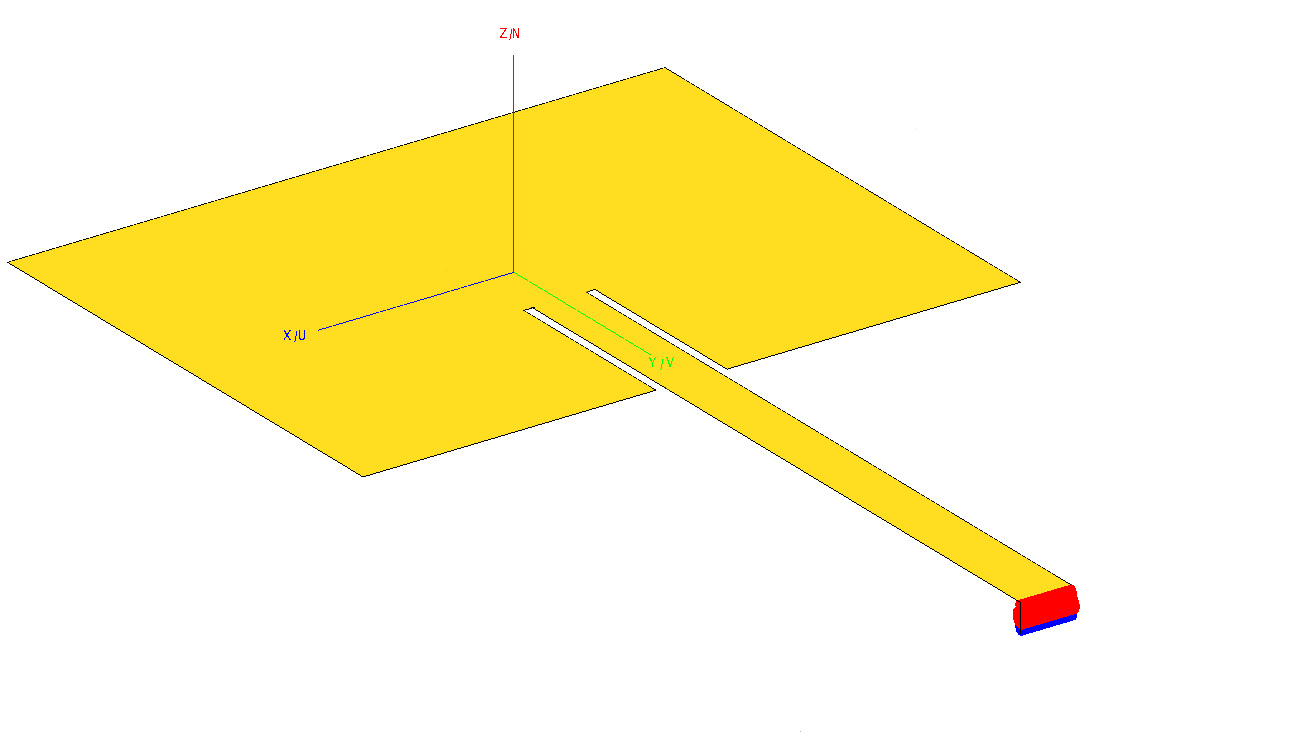
\includegraphics[width=\linewidth]{A_Cad.jpg}
  \caption{Modello CADFEKO dell'antenna con inset feed}
  \label{fig:A_Cad}
\end{figure}
Il modello è stato realizzato su un piano di massa infinito: questo permette di ridurre i tempi di simulazione. In particolare, i bordi di un substrato reale (con dimensioni finite) si comporterebbero anch'essi come elementi radianti, aumentando i tempi  di calcolo.
Con un piano infinito, questi effetti ai bordi vengono omessi. Di contro, non essendo possibile calcolare un'effettiva radiazione da parte del substrato, non si potranno fare osservazioni attendibili sui valori di potenza irradiata rapportata alla potenza dispersa nel mezzo dielettrico.\newline \newline
Simulato il modello, i primi risultati da discutere sono quelli riguardanti l'impedenza vista dal carico (Figura\ref{fig:A_impedenza}) e il coefficiente di riflessione $S_{11}$(Figura  \ref{fig:A_S11}).

 \begin{figure}[h!]
  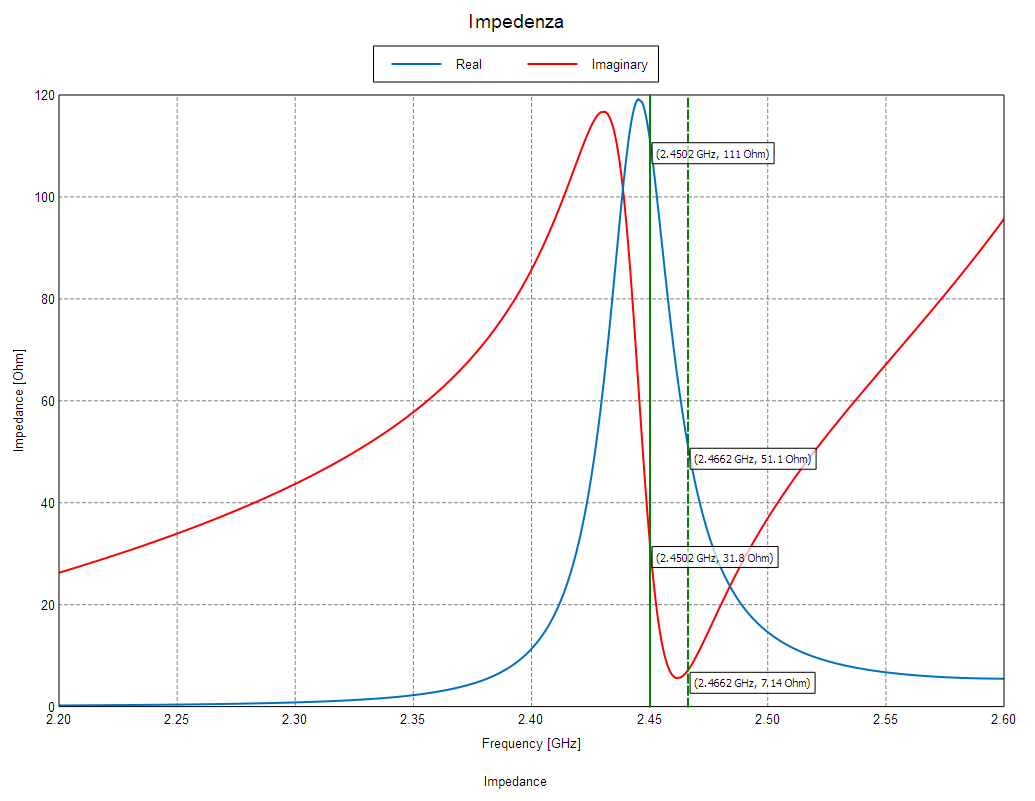
\includegraphics[width=\linewidth]{A_impedenza.png}
  \caption{Impedenza ($Re +Im$) vista dal carico, in funzione della frequenza[GHz]}
  \label{fig:A_impedenza}
\end{figure}
\begin{figure}[h!]
  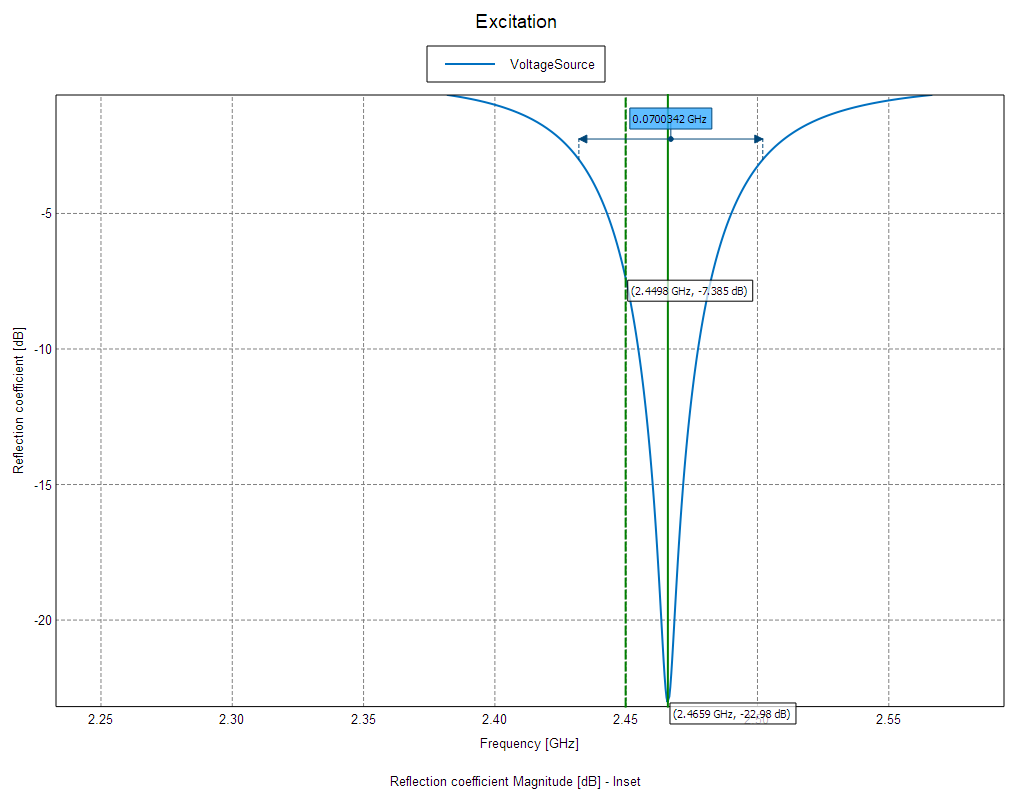
\includegraphics[width=\linewidth]{A_S11.png}
  \caption{$S_{11} $[dB] in funzione della frequenza [GHz] }
  \label{fig:A_S11}
\end{figure}
Il grafico di $S_{11}$ mostra il picco a minima riflessione centrato in  2.466 GHz con una banda a -3dB di 70MHz. La banda frazionaria risulta 2.8\% che è un valore tipico per questa
antenna.\newline Il risultato non è però ottimale: di fatto si sta cercando l'adattamento di impedenza con una frequenza di centro banda a 2.450 GHz.Questo indica che il carico non è abbastanza adattato alla linea di alimentazione.\newline
In Figura \ref{fig:A_impedenza} sono evidenziati i valori di impedenza visti dal generatore a 2.450 GHz e a 2.466 GHz. Per il punto di alimentazione scelto il carico non è ancora abbastanza adattato, e risulta $111 \;\Omega$.
%------------------------------------------------

\begin{figure}[h!]
  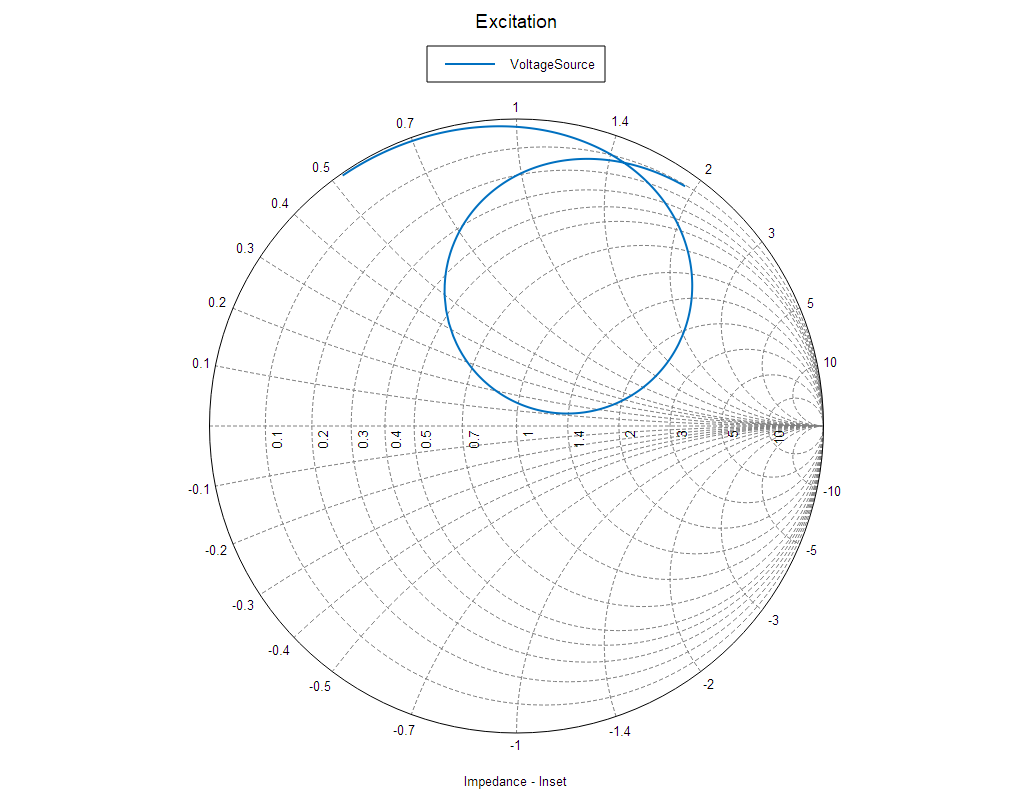
\includegraphics[width=\linewidth]{A_Smith.png}
  \caption{$S_{11} $ sulla carta di Smith,in funzione della frequenza}
  \label{fig:A_Smith}
\end{figure}

\begin{figure}[h!]
  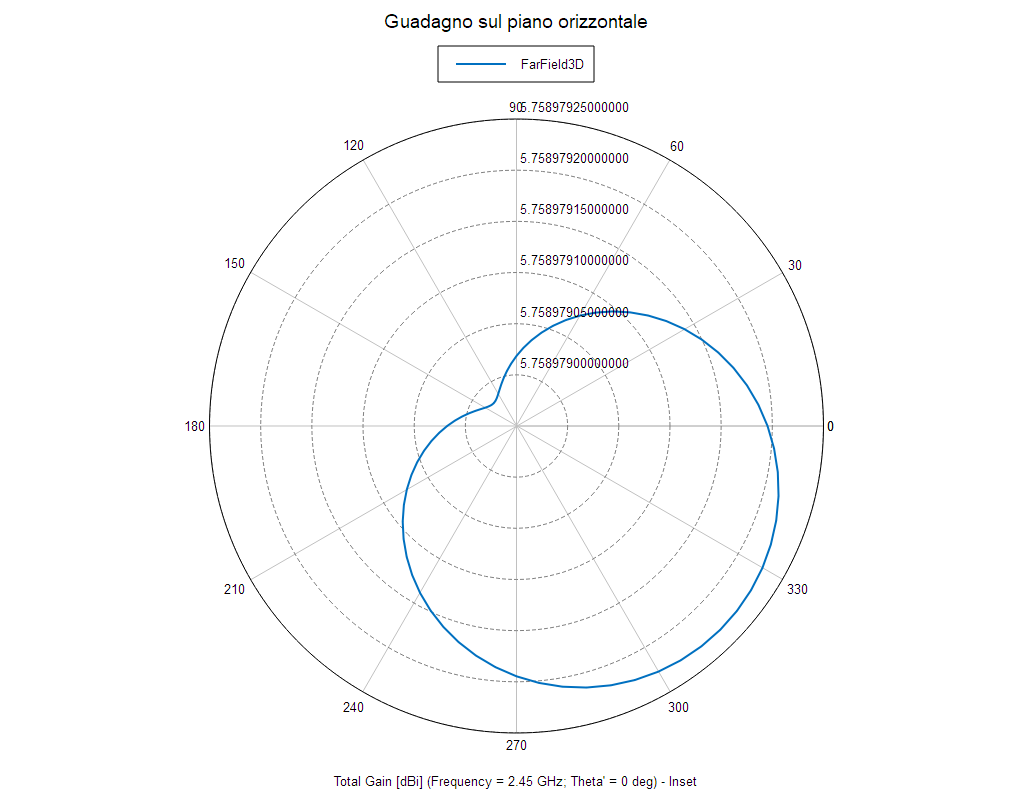
\includegraphics[width=\linewidth]{A_orizzontale.png}
  \caption{Ddr Guadagno [dBi], piano orizzontale}
  \label{fig:A_orizzontale}
\end{figure}

\begin{figure}[h!]
  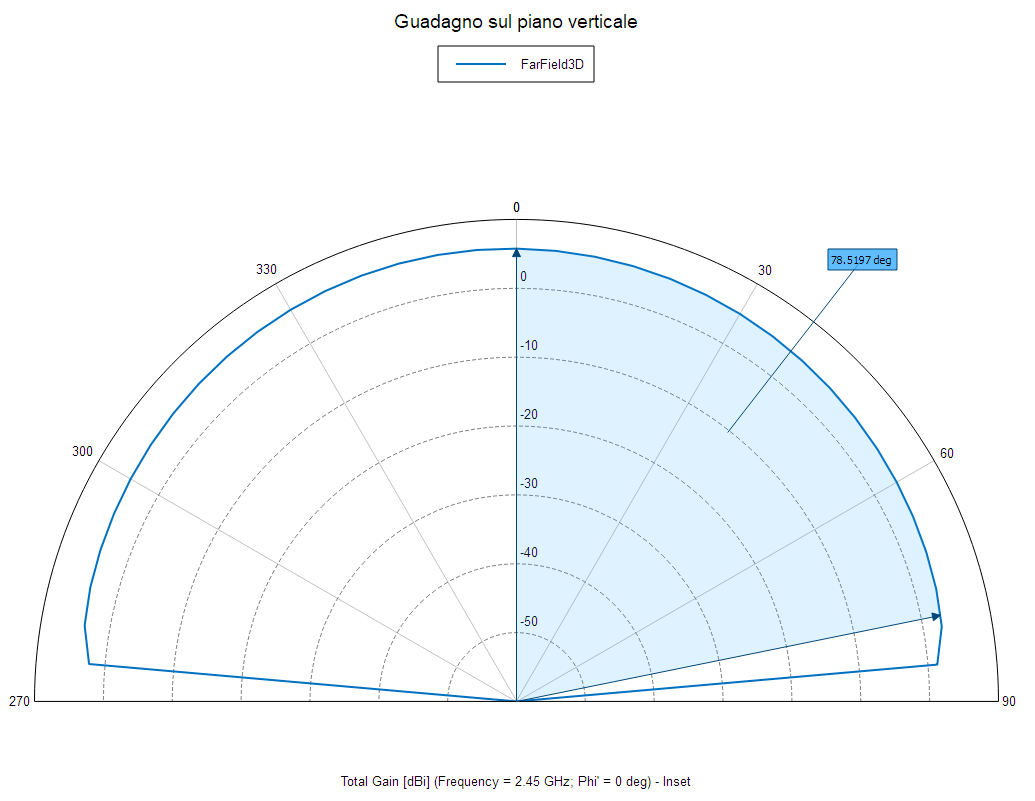
\includegraphics[width=\linewidth]{A_verticale.png}
  \caption{Ddr Guadagno [dBi] e apertura a -3dB, piano verticale}
  \label{fig:A_verticale}
\end{figure}

\subsection*{Trasformatore in $\frac{\lambda}{4}$ ed Inset Feed }
 \begin{figure}[h!]
  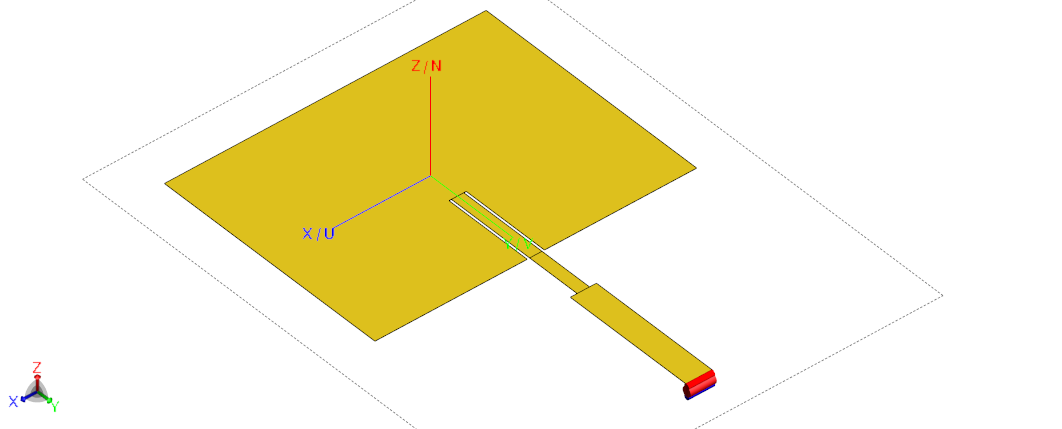
\includegraphics[width=\linewidth]{A1_Cad.png}
  \caption{Modello CADFEKO dell'antenna con inset feed combinato a trasformatore $\frac{\lambda}{4}$}
  \label{fig:A1_Cad}
\end{figure}
Per tentare di migliorare l'adattamento di impedenza ottenuto si è realizzato un secondo modello con le stesse caratteristiche del primo, dove però la linea di alimentazione a $50\Omega$ è stata combinata con un trasformatore in $\frac{\lambda}{4}$.
In questo modo si vuole adattare l'alimentazione al carico visto sul punto di inserzione il cui valore era dato dall'equazione \ref{eq:Rin}. \newline Osservando il grafico in Figura \ref{fig:A_impedenza}, il valore reale dell'impedenza raggiunge i $111 \Omega$ a 2.45 GHz. Si realizza quindi una sezione  in $\frac{\lambda}{4}$ di impedenza :
\begin{equation}
Z_{0}=\sqrt{Z_{C}R_{in}}=74.5 \Omega
\end{equation}
Durante le simulazioni sono state in oltre effettuati alcuni aggiustamenti alle dimensioni del modello  per ottenere un miglior risultato.Le variazioni sono riportate in tabella, comparati con i valori calcolati.
\begin{center}
\begin{tabular}{ |c|c|c|c| } 
 \hline
 W & L & $\rightarrow W$ & $\rightarrow L$\\ 
 37.3 mm& 27.8 mm & 41 mm & 28.8 \\ 
 \hline
\end{tabular}
\end{center}
In Figura \ref{fig:A1_Cad} è riportata la geometria del modello simulato mentre in Figura \ref{fig:A1_S11} è riportato il grafico di Return Loss.

\begin{figure}[h!]
  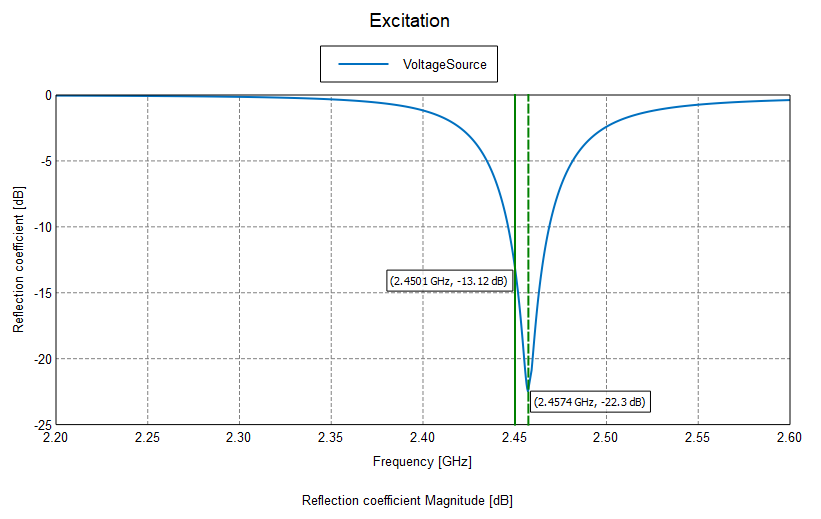
\includegraphics[width=\linewidth]{A1_S11.png}
  \caption{$S_{11} $[dB] in funzione della frequenza [GHz] }
  \label{fig:A1_S11}
\end{figure}
Con queste modifiche si è ottenuto un miglior adattamento sul carico dell'antenna e quindi circa -10 dB ulteriori del return loss attorno alla frequenza centrale. (Figura \ref{fig:A1_impedenza}),
 \begin{figure}[h!]
  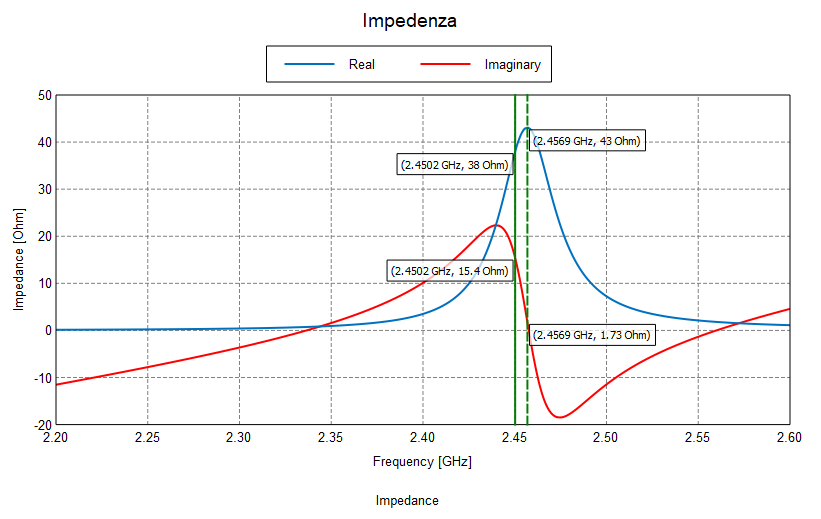
\includegraphics[width=\linewidth]{A1_impedenza.png}
  \caption{Impedenza ($Re +Im$) vista dal carico, in funzione della frequenza[GHz]}
  \label{fig:A1_impedenza}
\end{figure}
\begin{figure}[h!]
  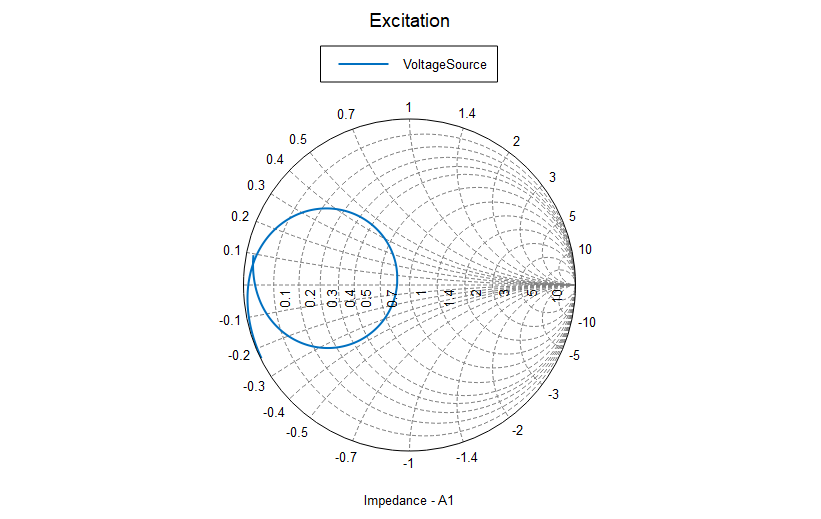
\includegraphics[width=\linewidth]{A1_Smith.png}
  \caption{$S_{11} $ sulla carta di Smith,in funzione della frequenza }
  \label{fig:A1_Smith}
\end{figure}

In seguito sono riportati i risultati relativi al guadagno dell'antenna e i diagrammi di radiazione.

\begin{figure}[h!]
  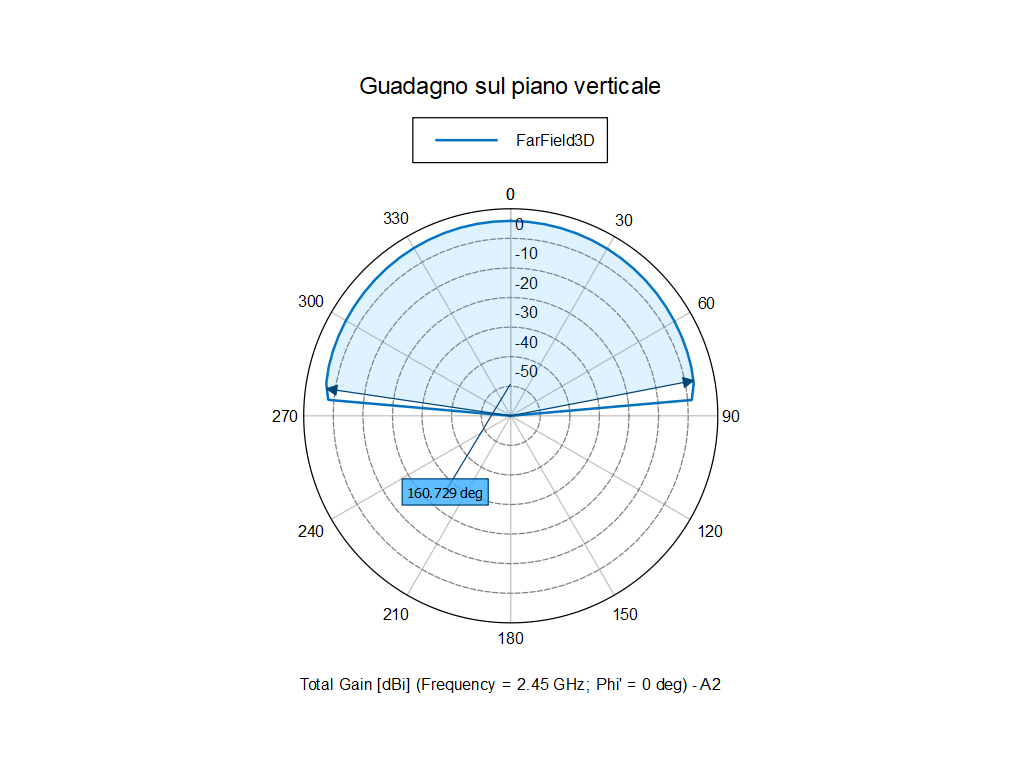
\includegraphics[width=\linewidth]{A1_verticale.png}
  \caption{Ddr Guadagno [dBi] e apertura a -3dB, piano verticale}
  \label{fig:A1_verticale}
\end{figure}
\begin{figure}[h!]
  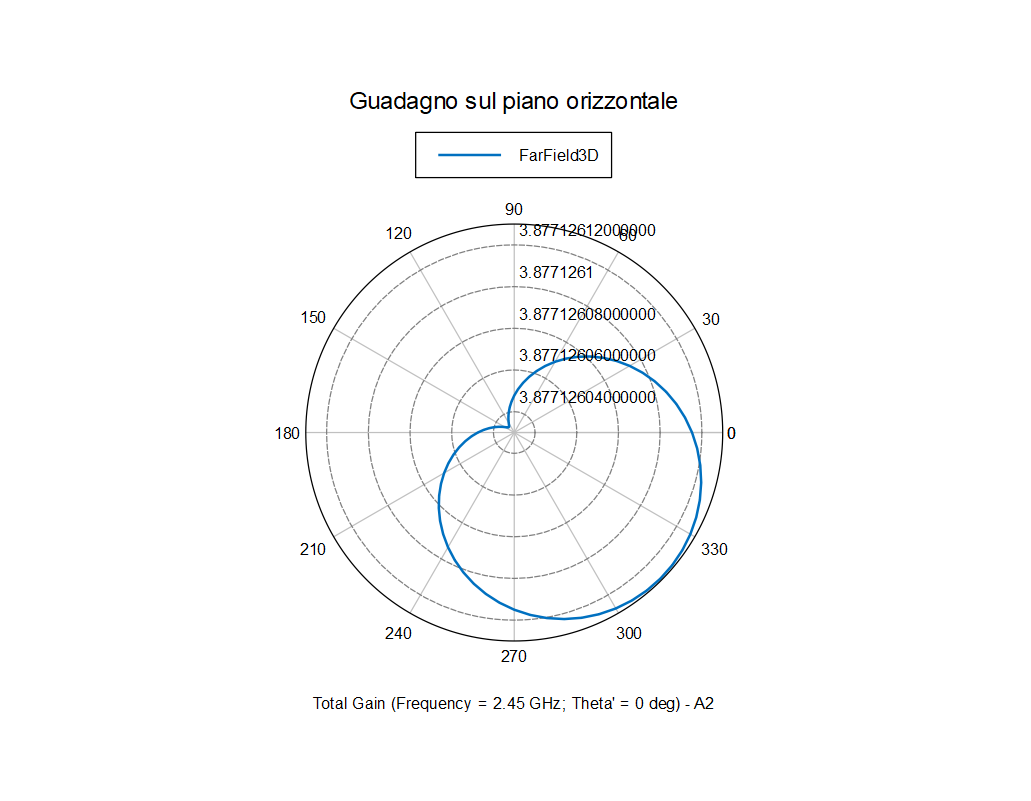
\includegraphics[width=\linewidth]{A1_orizzontale.png}
  \caption{Ddr Guadagno [dBi], piano orizzontale}
  \label{fig:A1_orizzontale}
\end{figure}


Il guadagno sul piano verticale raggiunge un massimo di 5.9 dBi, con un apertura a -3dB di circa 160.7$^\circ$
Il diagramma di radiazione ottenuto è quello tipico di un'antenna patch rettangolare.
Questo verrà confrontato con il diagramma Broadside dell'array a 4 elementi.


\section{Array Broadside}
\begin{figure}[h!]
  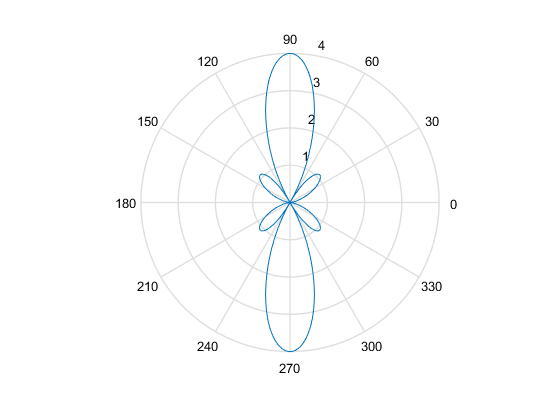
\includegraphics[width=\linewidth]{Array4E_matlab}
  \caption{Diagramma Broadside per un array a 4 elementi calcolato con Matlab}
  \label{fig:Array4E_matlab}
\end{figure}


\subsection*{Feed Network}
\begin{figure}[h!]
  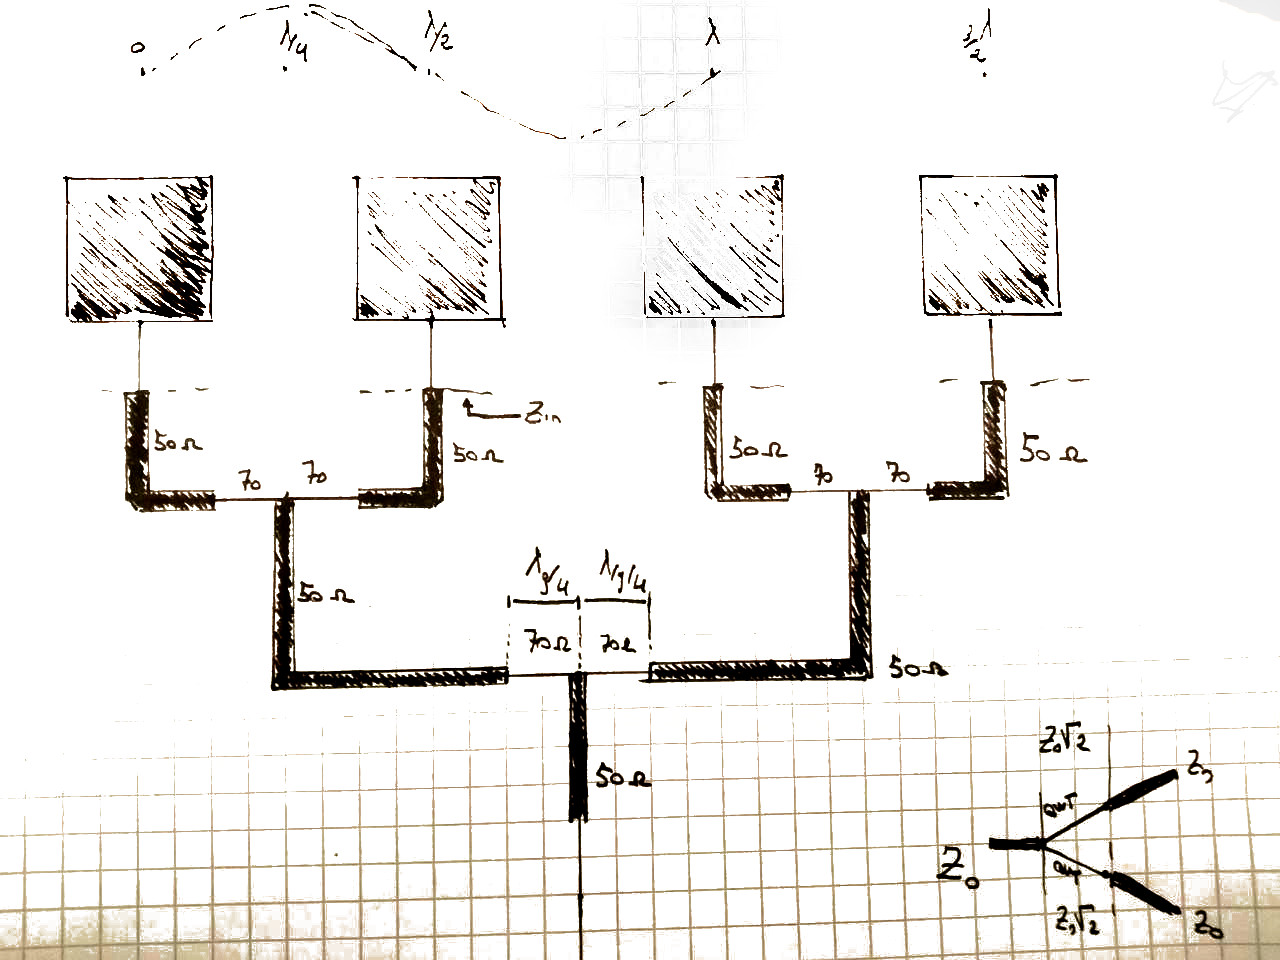
\includegraphics[width=\linewidth]{Array4E_Schema.jpg}
  \caption{Schema del corporate feed per 4 elementi}
  \label{fig:Array4E_Schema}
\end{figure}
Dal singolo elemento si sviluppa l'array 4x1 per ottenere una radiazione broadside.
Il primo passo è calcolare l'array factor che è dato da:
\begin{equation}
AF(\phi)=\sum_{m=1}^{N} a_{m} e^{jm \phi}
\end{equation}
dove $\phi=kd\cos\theta$.\newline
Si sceglie una distanza fra gli elementi  $d=\frac{\lambda}{2}$ e si alimenta in fase l'array.
Il pattern di radiazione calcolato con Matlab e riportato in Figura \ref{fig:Array4E_matlab}.
\begin{figure}[h]
  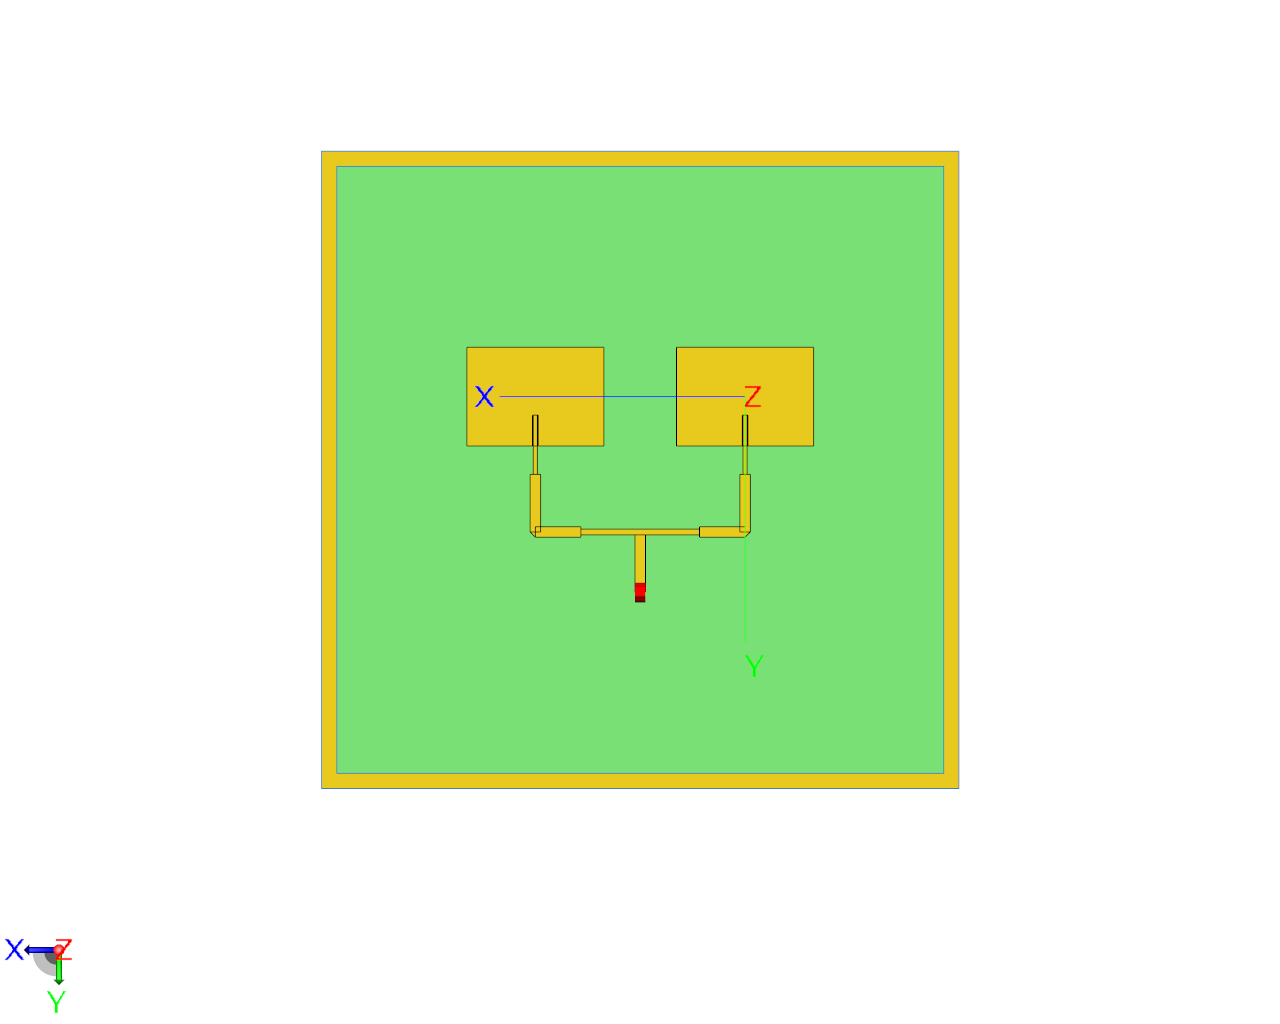
\includegraphics[width=\linewidth]{Array2E_Cad.png}
  \caption{Modello FEKO dell'array per 2 elementi}
  \label{fig:Array2E_Cad}
\end{figure}

\begin{figure}[h!]
  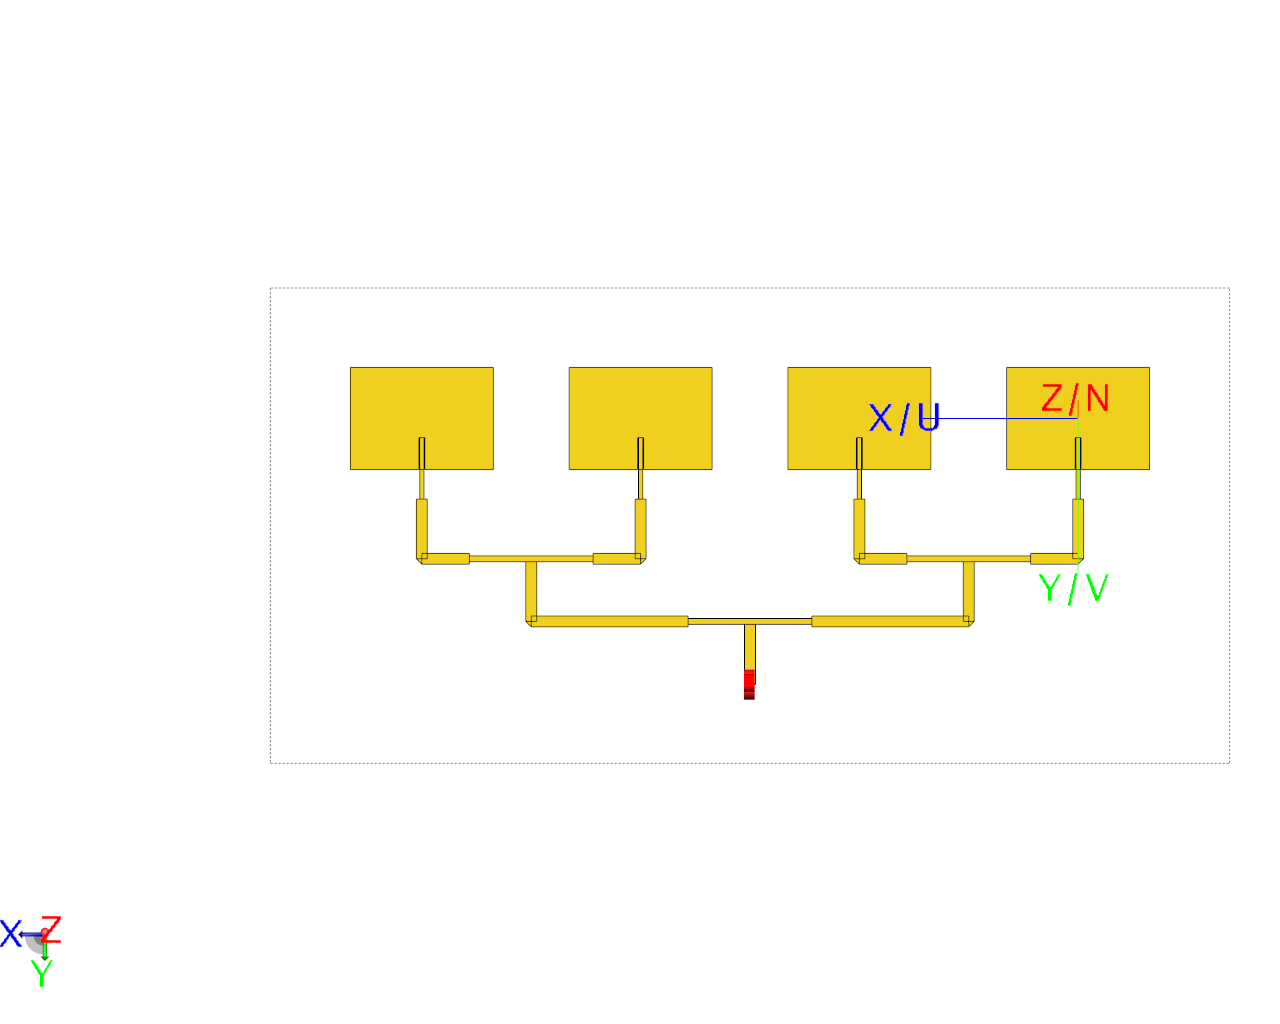
\includegraphics[width=\linewidth]{Array4E_Cad.png}
  \caption{Modello FEKO dell'array per 4 elementi}
  \label{fig:Array4E_Cad}
\end{figure}

La rete di alimentazione è composta da una combinazione di divisori a 3dB che distribuiscono la potenza alle 4 antenne.
Il divisore di potenza divide equamente la potenza senza perdite ma l'impedenza vista dall'ingresso sulle due uscite non è adattata ed equivale a $2Z_{0}$.
Si rende necessario quindi aggiungere dei trasformatori in $\frac{\lambda}{4}$ da $70 \Omega$ per adattare le uscite.
\newline
Lo schema dell'intera rete è riportata in Figura \ref{fig:Array4E_Schema}, mentre in Figura \ref{fig:Array4E_Cad} è riportato il relativo modello  realizzato su FEKO Student.



I risultati della simulazione mostrano la radiazione broadside  dell'antenna (molto direttiva, tipo "Pencil Beam") con un guadagno massimo di circa 10.7 dBi  (in $\theta =0 \;\; \forall \phi$).

\begin{figure}[h]
  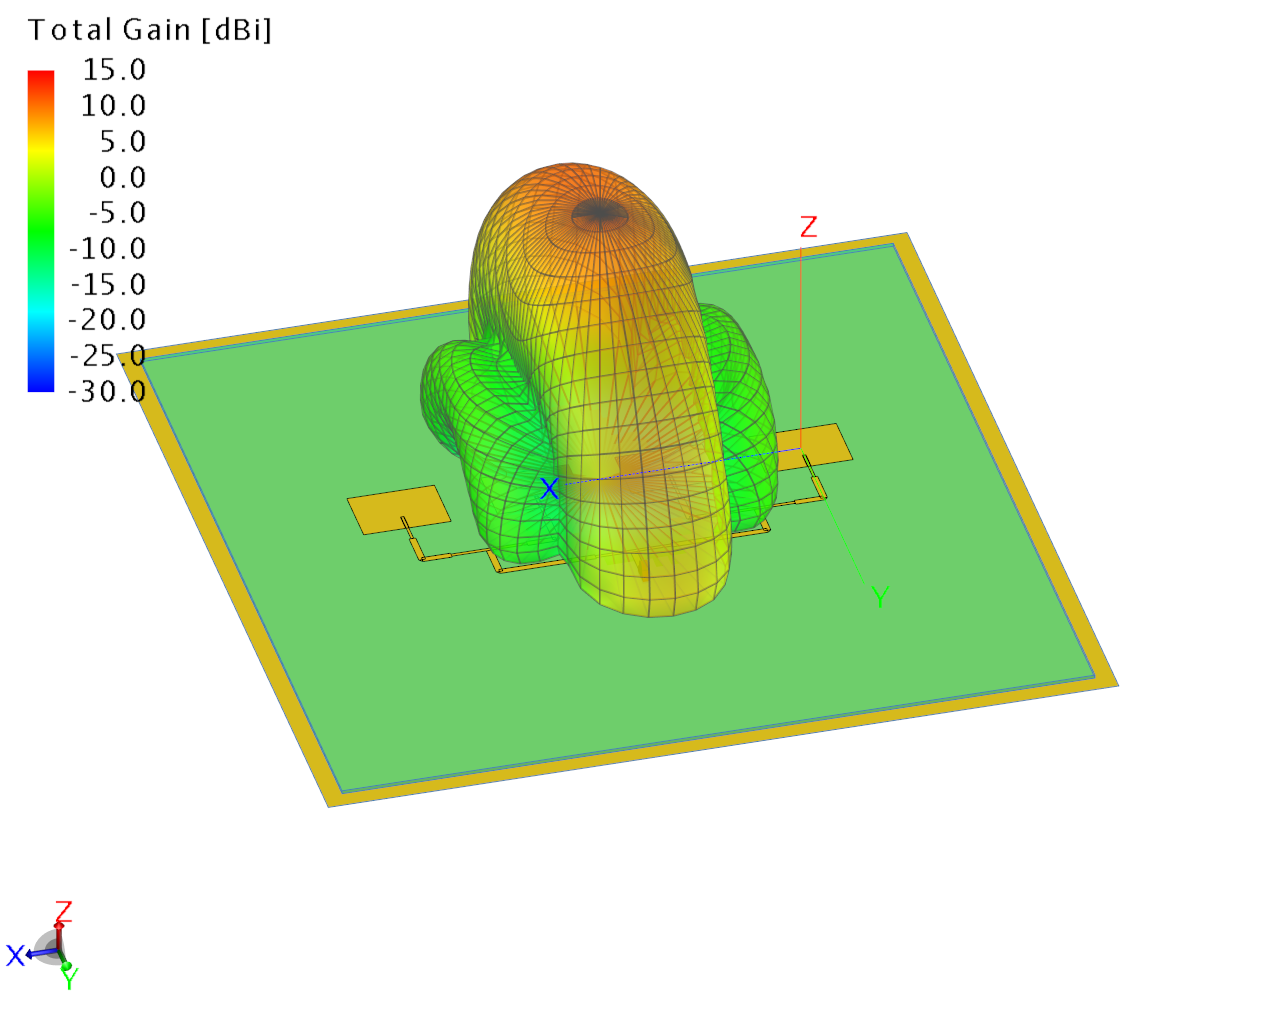
\includegraphics[width=\linewidth]{Array4E_Gain.png}
  \caption{Guadagno 3D [dBi]}
  \label{fig:Array4E_Gain}
\end{figure}
\begin{figure}[h]
  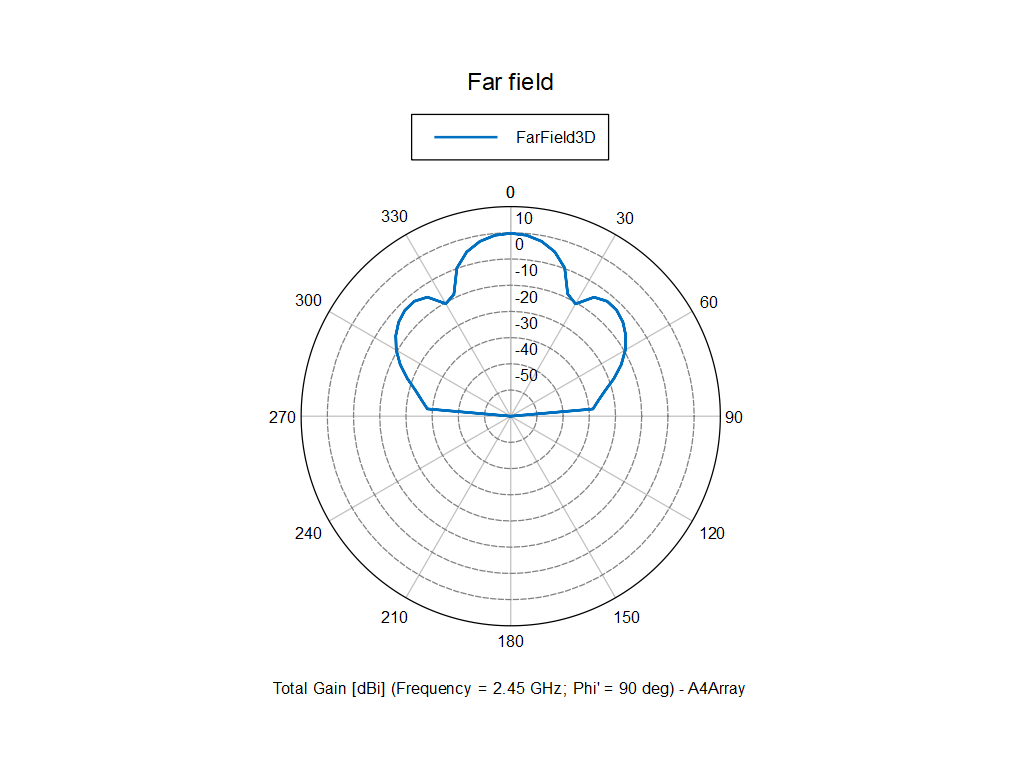
\includegraphics[width=\linewidth]{Array4E_verticale.png}
  \caption{Ddr Guadagno [dBi], piano verticale}
  \label{fig:Array4E_verticale}
\end{figure}

In Figura \ref{fig:Array4E_S11}, il notch della curva S11 non raggiunge i valori ottenuti in precedenza. \newline
La complessità della rete di alimentazione richiede che venga  nuovamente "riassestato" l'adattamento tra l'alimentazione e l'intero carico visto da quest'ultima.\
\begin{figure}[h]
  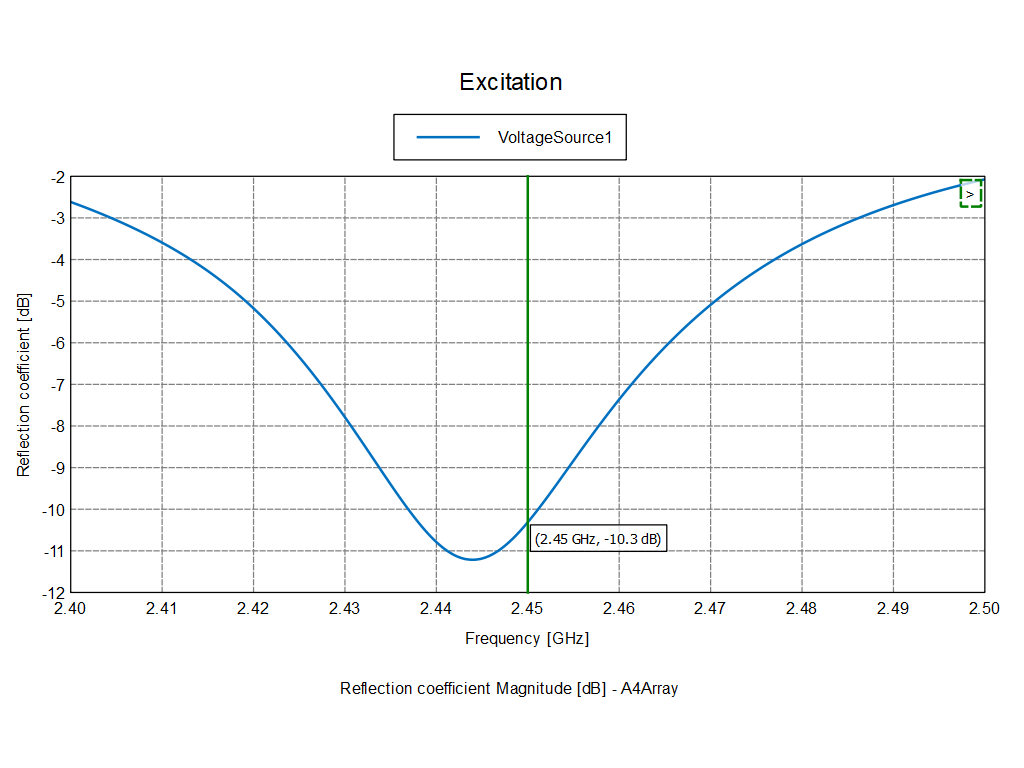
\includegraphics[width=\linewidth]{Array4E_S11.png}
  \caption{$S_{11} $[dB] in funzione della frequenza [GHz]}
  \label{fig:Array4E_S11}
\end{figure}

\begin{figure}[h]
  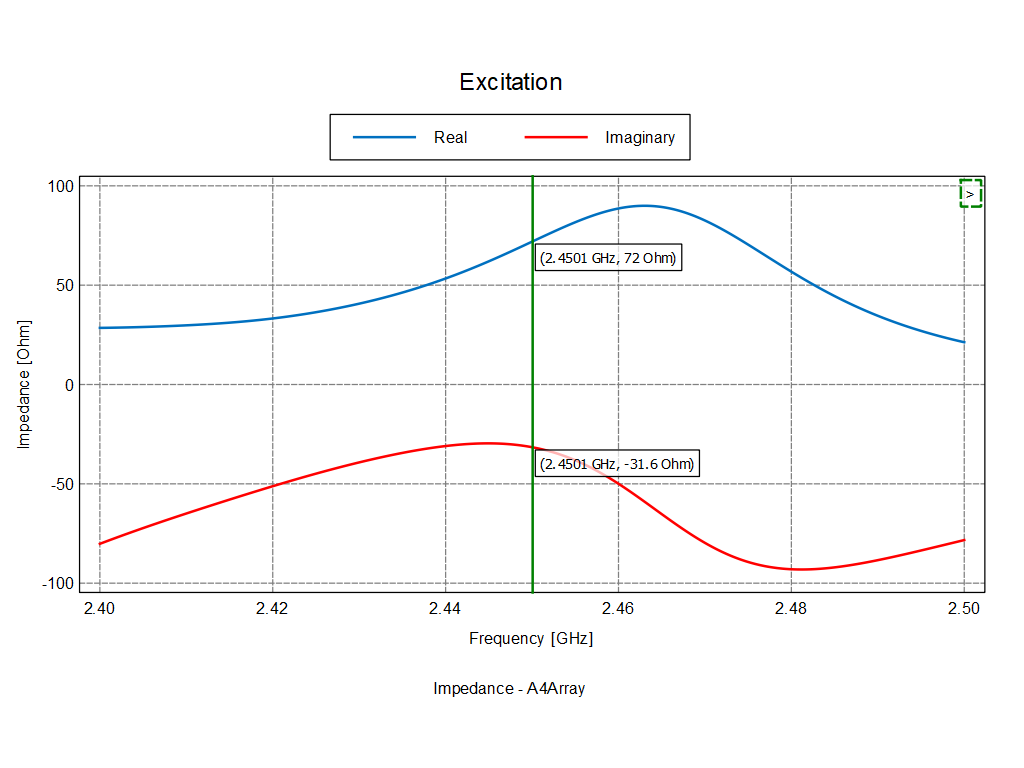
\includegraphics[width=\linewidth]{Array4E_impedenza.png}
  \caption{Impedenza ($Re +Im$) vista dal carico, in funzione della frequenza[GHz]}
  \label{fig:Array4E_impedenza}
\end{figure}

%------------------------------------------------




%----------------------------------------------------------------------------------------
%	REFERENCE LIST
%----------------------------------------------------------------------------------------
%
\begin{thebibliography}{99} % Bibliography - this is intentionally simple in this template

\bibitem{balanis} C. A. Balanis, \emph
{Antenna Theory Analysis and Design}.
\bibitem{ning} Zhi Ning Chen and Michael Y. W. Chia, \emph
{Broadband Planar Antennas, Design and Applications}.

\bibitem{Pozar} Pozar D.M., \emph
{Microwave engineering}.
\bibitem{matching} Sonia Sharma, C. C. Tripathi and Rahul Rishi, \emph
{Impedance Matching Techniques for Microstrip
Patch Antenna}.
\bibitem{tesi} Andrea Cupido, \emph
{PROGETTAZIONE ASSISTITA AL CALCOLATORE DI ANTENNE “PATCH”}.

\end{thebibliography}

%----------------------------------------------------------------------------------------

\end{document}
